\documentclass[aspectratio=169,
hyperref={colorlinks,urlcolor=blue}
]{beamer}


%\usetheme{Pittsburgh}
\usetheme{default}
\usepackage{colortbl}%colored tables
%For using helvetica font:
\usepackage[scaled]{helvet}
\usepackage[T1]{fontenc}
\renewcommand\familydefault{\sfdefault}
\urlstyle{same} %sets the fonts for urls
\usepackage{pdfpages}
\usepackage{siunitx}
\usepackage{caption}
\usepackage{pifont}%for dings
\usepackage{pgfplots}%for 3d plotting
\pgfplotsset{compat = newest}
\usepackage{mathtools}%box in align env \Aboxed
\usepackage[american,smartlabels]{circuitikz}%for drawing circuits
\usepackage{multimedia}
\usepackage{animate}
\usepackage{xcolor}


\usetikzlibrary{arrows}
\usetikzlibrary {3d} 
\usetikzlibrary{decorations.markings, math}
\usetikzlibrary{intersections, pgfplots.fillbetween}
\usetikzlibrary {shapes.geometric} 


%\definecolor{myblue}{RGB}{5, 34, 150}
\definecolor{myblue2}{RGB}{5, 34, 150}
\definecolor{myblue}{RGB}{0,36,82}
\definecolor{myred}{RGB}{207, 2, 13}
\definecolor{mygreen}{RGB}{0, 158, 11}
\definecolor{myyellow}{RGB}{220,220,0}
\definecolor{qblue}{RGB}{0,36,82}
\definecolor{qgold}{RGB}{250,189,15}
\definecolor{qred}{RGB}{185,14,49}
\definecolor{cblue}{rgb}{0.13, 0.67, 0.8}
\definecolor{corange}{rgb}{0.8, 0.34, 0.0}
\definecolor{cpurple}{rgb}{0.54, 0.29, 0.42}

%%%%%%%%%%%% General settings
\setbeamercolor{frametitle}{fg=black}
\setbeamercolor{title}{fg=black}
\setbeamercolor{author}{fg=myblue2}

\beamertemplatenavigationsymbolsempty %no navigation controls at bottom of slides
%\setbeamertemplate{footline}[frame number]
\usefonttheme{professionalfonts} 
\setbeamerfont{title}{series=\bfseries,parent=structure}
\setbeamerfont{frametitle}{series=\bfseries,parent=structure}

%%%%%%%%%%%%Lists
\setbeamertemplate{itemize item}[circle] %{\color{myblue}$\circ$}
\setbeamertemplate{itemize subitem}{\color{myblue2}$\circ$}
\setbeamertemplate{itemize subsubitem}{\color{myblue2}$\cdot$}
\setbeamercolor{itemize item}{bg=myblue2,fg=myblue2}
\setbeamercolor{enumerate item}{bg=myblue2,fg=myblue2}
%%%%%%%%%%%%%%%%%%%%%%%%%%%%

%%%%%%%%%%%%Blocks
\setbeamertemplate{blocks}[rounded]
%Default block
\setbeamercolor{block title}{bg=myblue2, fg=white}
\setbeamercolor{block body}{bg=myblue2!10}
\setbeamerfont{block body}{size=\scriptsize}
\setbeamerfont{block title}{size=\scriptsize}
%Alert block
\setbeamercolor{block title alerted}{bg= myblue2, fg=white}
\setbeamercolor{block body alerted}{bg=myblue2!10}
\setbeamerfont{block body alerted}{size=\scriptsize}
\setbeamerfont{block title alerted}{size=\scriptsize}
%example block
\setbeamercolor{block title example}{bg=mygreen, fg=white}
\setbeamercolor{block body example}{bg=mygreen!10}
\setbeamerfont{block body example}{size=\scriptsize}
\setbeamerfont{block title example}{size=\scriptsize}
%%%%%%%%%%%%%%%%55


%%%%%%%%%%%%Figures and captions
\captionsetup{font=scriptsize,labelfont=scriptsize}
%\setbeamertemplate{caption}{\raggedright\insertcaption\par}
\newenvironment{capfig}[3]{\begin{figure}\includegraphics[width=#1\textwidth]{#2}\caption*{\textit{#3}}\end{figure}}{}

%\makeatother
%\setbeamertemplate{footline}
%{
%  \leavevmode%
%  \hbox{%
%  \begin{beamercolorbox}[wd=.4\paperwidth,ht=2.25ex,dp=1ex,center]{author in head/foot}%
%    \usebeamerfont{author in head/foot}\insertshortauthor
%  \end{beamercolorbox}%
%  \begin{beamercolorbox}[wd=.6\paperwidth,ht=2.25ex,dp=1ex,center]{title in head/foot}%
%    \usebeamerfont{title in head/foot}\insertshorttitle\hspace*{3em}
%    \insertframenumber{} / \inserttotalframenumber\hspace*{1ex}
%  \end{beamercolorbox}
%  }%
%  \vskip0pt%
%}
%\makeatletter

\makeatother
\setbeamertemplate{footline}
{
  \leavevmode%
  \hbox{%
\begin{beamercolorbox}[wd=.27\paperwidth,ht=2.25ex,dp=1ex,center]{author in head/foot}%
    \color{black}{\insertinstitute}
\end{beamercolorbox}
  \begin{beamercolorbox}[wd=.27\paperwidth,ht=2.25ex,dp=1ex,center]{author in head/foot}%
    \color{black}{\inserttitle}
  \end{beamercolorbox}%
  \begin{beamercolorbox}[wd=.27\paperwidth,ht=2.25ex,dp=1ex,center]{title in head/foot}%
    \color{black}{\insertshortauthor}
  \end{beamercolorbox}
  \begin{beamercolorbox}[wd=.27\paperwidth,ht=2.25ex,dp=1ex,center]{title in head/foot}%
    \hspace{.28\paperwidth}\color{black} \insertframenumber{} / \inserttotalframenumber\hspace*{1ex}
  \end{beamercolorbox}
  }%
  \vskip0pt%
}
\makeatletter

\setbeamertemplate{title page}
{
  \begin{tikzpicture}[remember picture,overlay]
    \def\barh{4}%15
  
    \draw[color=myblue2,line width=\barh] ([yshift=-0.5*\barh]current page.north west) -- ([yshift=-0.5*\barh,xshift=-0.67\paperwidth]current page.north east);
    \draw[color=myblue2,line width=\barh] ([yshift=-0.5*\barh,xshift=-0.67\paperwidth]current page.north east) -- ([yshift=-0.5*\barh,xshift=-0.34\paperwidth]current page.north east);
    \draw[color=myblue2,line width=\barh] ([yshift=-0.5*\barh,xshift=-0.34\paperwidth]current page.north east) -- ([yshift=-0.5*\barh]current page.north east); 
  
    \draw[color=myblue2,line width=\barh] ([yshift=0.5*\barh]current page.south west) -- ([yshift=0.5*\barh,xshift=-0.67\paperwidth]current page.south east);
    \draw[color=myblue2,line width=\barh] ([yshift=0.5*\barh,xshift=-0.67\paperwidth]current page.south east) -- ([yshift=0.5*\barh,xshift=-0.34\paperwidth]current page.south east);
    \draw[color=myblue2,line width=\barh] ([yshift=0.5*\barh,xshift=-0.34\paperwidth]current page.south east) -- ([yshift=0.5*\barh]current page.south east);
    %\node[left] at (current page.east) {
    %
\includegraphics[scale=0.1]{figures/coverpage}
    %};
  \end{tikzpicture}
  
  \usebeamerfont{title}\usebeamercolor[fg]{title}\inserttitle\par
  \usebeamerfont{subtitle}\usebeamercolor[fg]{subtitle}\insertsubtitle\par
  \vspace{2cm}
  \usebeamerfont{author}\usebeamercolor[fg]{author}\insertauthor\par
  \usebeamerfont{institute}\usebeamercolor[fg]{author}\insertinstitute\par
  \usebeamercolor[fg]{author}\par
  \usebeamercolor[fg]{titlegraphic}\inserttitlegraphic

} 

\setbeamertemplate{frametitle}{%
    \nointerlineskip%
        \par\hspace*{-\dimexpr0.5\paperwidth-0.5\textwidth}\textcolor{myblue2}{\rule{0.33\paperwidth}{6pt}}\textcolor{myblue2}{\rule{0.33\paperwidth}{6pt}}\textcolor{myblue2}{\rule{0.34\paperwidth}{6pt}} 
    \begin{beamercolorbox}[wd=\paperwidth,ht=0.75cm,dp=0.6ex]{frametitle}
        \hspace*{0.5cm}\strut\usebeamerfont{frametitle}\insertframetitle\strut
        %\hrule
    \end{beamercolorbox}%
    %%Line below:
%\par\hspace*{-\dimexpr0.5\paperwidth-0.5\textwidth}\textcolor{myblue}{\rule{\paperwidth}{0.4pt}}
     % <-- calculation of left margin width + rule
     %\textcolor{red}{\noindent\rule{\paperwidth}{2pt}}
}


%%%%%%%%%%%%Frame templates

%Slide with title
\newenvironment{titleframe}[1]
{\begin{frame}\frametitle{#1}\end{frame}}
{}

%Slide with title and itemize list:
\newenvironment{bulletframe}[1]
{\begin{frame}{#1} \itemize}
{\enditemize \end{frame}}

%Slide with two columns 50/50
\newenvironment{twocolframe}[3]
{\begin{frame}{#1}
 \begin{columns}[T]
 \column{0.5\textwidth}#2
 \column{0.5\textwidth}#3
 \end{columns}\end{frame}}{}

%Slide with two columns 60/40 <<<<<<<<<<<<<<<<<<<<<<  This one!
\newenvironment{twocolframesf}[3]
{\begin{frame}{#1}
 \begin{columns}[T]
 \column{0.6\textwidth}#2
 \column{0.4\textwidth}#3
 \end{columns}\end{frame}}{}
 
%Slide with two columns 70/30
\newenvironment{twocolframest}[3]
{\begin{frame}{#1}
 \begin{columns}[T] 
 \column{0.7\textwidth}#2
 \column{0.3\textwidth}#3
 \end{columns}\end{frame}}{} 
 
%Slide with two columns 40/60
\newenvironment{twocolframefs}[3]
{\begin{frame}{#1}
 \begin{columns}[T] 
 \column{0.4\textwidth}#2
 \column{0.6\textwidth}#3
 \end{columns}\end{frame}}{}
 
%Slide with two columns 70/30
\newenvironment{twocolframets}[3]
{\begin{frame}{#1}
 \begin{columns}[T] 
 \column{0.3\textwidth}#2
 \column{0.7\textwidth}#3
 \end{columns}\end{frame}}{} 

 
%Colloquium speaker (title, abstract, picture file, speaker name)
\newenvironment{colloquium}[5]
{
\begin{frame}{Colloquium: Friday 1:30pm in Stirling A}
\begin{columns}[T] 
 \column{0.8\textwidth}
 \textbf{#1}\\
 #2
 \column{0.2\textwidth}
 \capfig{#3}{#4}{#5}
 \end{columns}
\end{frame}
}
{} 

%%%%%%%%%%%%%Set Hyperref colors


\hypersetup{
  colorlinks=true,
  linkcolor=blue,    
  urlcolor=blue,     
  citecolor=blue      
}
%%%%%%%%%%%%%TOC bolding
\setbeamerfont{section in toc}{series=\bfseries}





%Frames:
% \twocolframesf 60/40 (fs, st, ts) 
% \titleframe
% bulletframe

%%%%%%%%%%%%%%%%%%%%%%%%%
%%%%%% START OF PRESENTATION %%%%%%
%%%%%%%%%%%%%%%%%%%%%%%%%

\title{Newton's Laws}
\institute{Newton, Forces, and Free Body Diagrams}
\author{Building Models to Describe our World}

\begin{document}

\begin{frame}
\titlepage
\thispagestyle{empty}

\begin{textblock*}{5cm}(11cm,4cm)
    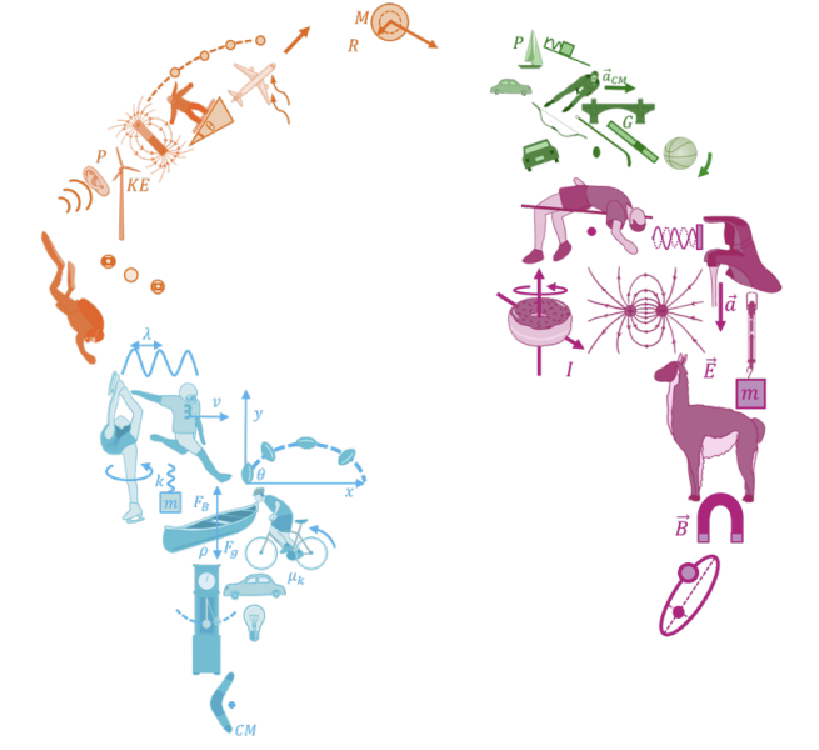
\includegraphics[width=4cm]{../figures/BMDW/logo}
\end{textblock*}

\end{frame}

\subsection{Forces}
\label{subsec:forces}
\begin{bulletframe}{Forces}
\item There is no such thing as a force.
\item These are a mathematical tool that allows us to describe the motion of objects. 
\item We represent them with a vector, as they have a magnitude and a direction.
\item We can use a spring scale to define the magnitude and direction of a force.
\item One issue is that we have some intuition about what a force feels like; it’s better to apply rules for modelling forces, rather than trying to guess and apply intuition. Some concepts are counter-intuitive.
\begin{itemize}
\item With practice, you will develop intuition about whether to include a specific force, not about what a force really is. The ``physics intuition'' is about getting comfortable applying the rules, not about understanding them. Nobody ``understands'' the rules.
\end{itemize}

\end{bulletframe}

%%%%%%%%%%%%%%%%%%%%%%%%%%%%%%%%
\subsection{Group Exercise: FBD 1}
\label{subsec:groupfbd1}
\begin{frame}{Group exercise: Draw FBD for each object}
 \begin{columns}[T]
 \column{0.5\textwidth}
\begin{center}
\begin{tikzpicture}[scale=1]
\tikzmath{
\L=1;
}
\pgfmathsetmacro{\hval}{0.85}
\scalebox{1.0}{
\node at (0,0) {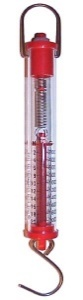
\includegraphics[scale=0.5]{../figures/NewtonsLaws/scale}};
\fill [black!50] (-\L/2,-\L-\hval) rectangle (\L/2,-\hval);
\fill (-\L,\hval) rectangle (\L,\hval+0.2);
\node at (0,-\L/2-\hval){$m$};

\fill (2*\L,\hval+0.1) circle(3pt) node[right=2pt]{ceiling};
\fill (2.5*\L,0) circle(3pt) node[right=2pt]{scale};
\fill (2*\L,-\L/2-\hval) circle(3pt) node[right=2pt]{mass};

}
\end{tikzpicture}
\end{center}
 \column{0.5\textwidth}
\begin{center}
\begin{tikzpicture}[scale=1]
\tikzmath{
\L=1;
}
\pgfmathsetmacro{\hval}{0.85}
\scalebox{1.0}{
\node at (0,\hval) {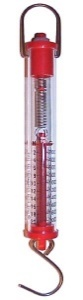
\includegraphics[scale=0.5]{../figures/NewtonsLaws/scale}};
\node at (0,-\hval) {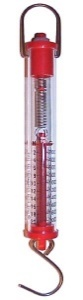
\includegraphics[scale=0.5]{../figures/NewtonsLaws/scale}};
\fill (-\L,2*\hval) rectangle (\L,2*\hval+0.2);
\fill [black!50] (-\L/2,-\L-2*\hval) rectangle (\L/2,-2*\hval);
\node at (0,-\L/2-2*\hval){$m$};

\fill (2*\L,2*\hval+0.1) circle(3pt) node[right=2pt]{ceiling};
\fill (2.5*\L,\hval) circle(3pt)node[right=2pt]{scale};
\fill (2*\L,-\hval) circle(3pt)node[right=2pt]{scale};
\fill (2.5*\L,-\L/2-2*\hval) circle(3pt)node[right=2pt]{mass};


}
\end{tikzpicture}
\end{center}
 \end{columns}
\begin{itemize}
\scriptsize
\item Assume the scales are massless.
\item Draw free body diagrams for the masses, scales and ceiling in both cases. (Draw little arrows around each point!).
\item Remember, all objects must have an acceleration of zero!
\item Be clear about what exerts a force on what!
\end{itemize}
\end{frame}


%%%%%%%%%%%%%%%%%%%%%%%%%%%%%%%%

\begin{frame}{Group exercise: Draw FBD for each object}
 \begin{columns}[T]
 \column{0.5\textwidth}
\begin{center}
\begin{tikzpicture}[scale=1]
\tikzmath{
\L=1;
\f=0.5;
}
\pgfmathsetmacro{\hval}{0.85}
\scalebox{1.0}{
\node at (0,0) {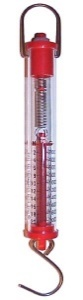
\includegraphics[scale=0.5]{../figures/NewtonsLaws/scale}};
\fill [black!50] (-\L/2,-\L-\hval) rectangle (\L/2,-\hval);
\fill (-\L,\hval) rectangle (\L,\hval+0.2);
\node at (0,-\L/2-\hval){$m$};

\fill (2*\L,\hval+0.1) circle(3pt);
\draw [-latex,line width=1.5,color=myred] (2*\L,\hval+0.1) -- +(0,\f) node[midway,right]{\scriptsize Force from building on ceiling};
\draw [-latex,line width=1.5] (2*\L,\hval+0.1) -- +(0,-\f) node[midway,right]{\scriptsize Force from scale on ceiling};
\fill (2.5*\L,-0.25*\hval) circle(3pt) ;
\draw [-latex,line width=1.5] (2.5*\L,-0.25*\hval) -- +(0,\f) node[midway,right]{\scriptsize Force from ceiling on scale};
\draw [-latex,line width=1.5] (2.5*\L,-0.25*\hval) -- +(0,-\f) node[midway,right]{\scriptsize Force from mass on scale};
\fill (2*\L,-\L/2-\hval) circle(3pt) ;
\draw [-latex,line width=1.5] (2*\L,-\L/2-\hval) -- +(0,\f) node[midway,right]{\scriptsize Force from scale on mass};
\draw [-latex,line width=1.5,color=myred] (2*\L,-\L/2-\hval) -- +(0,-\f) node[midway,right]{\scriptsize Force from gravity on mass};
}
\end{tikzpicture}
\end{center}
 \column{0.5\textwidth}
\begin{center}
\begin{tikzpicture}[scale=1]
\tikzmath{
\L=1;
\f=0.5;
}
\pgfmathsetmacro{\hval}{0.85}
\scalebox{1.0}{
\node at (0,\hval) {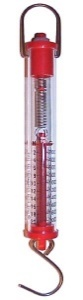
\includegraphics[scale=0.5]{../figures/NewtonsLaws/scale}};
\node at (0,-\hval) {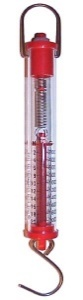
\includegraphics[scale=0.5]{../figures/NewtonsLaws/scale}};
\fill (-\L,2*\hval) rectangle (\L,2*\hval+0.2);
\fill [black!50] (-\L/2,-\L-2*\hval) rectangle (\L/2,-2*\hval);
\node at (0,-\L/2-2*\hval){$m$};

\fill (2*\L,2*\hval+0.1) circle(3pt) ;
\draw [-latex,line width=1.5,color=myred] (2*\L,2*\hval+0.1) -- +(0,\f) node[midway,right]{\scriptsize Force from building on ceiling};
\draw [-latex,line width=1.5] (2*\L,2*\hval+0.1) -- +(0,-\f) node[midway,right]{\scriptsize Force from scale on ceiling};
\fill (2.5*\L,\hval) circle(3pt);
\draw [-latex,line width=1.5] (2.5*\L,\hval) -- +(0,\f) node[midway,right]{\scriptsize Force from ceiling on scale};
\draw [-latex,line width=1.5] (2.5*\L,\hval) -- +(0,-\f) node[midway,right]{\scriptsize Force from scale on scale};
\fill (2*\L,-\hval) circle(3pt);
\draw [-latex,line width=1.5] (2*\L,-\hval)  -- +(0,\f) node[midway,right]{\scriptsize Force from scale on scale};
\draw [-latex,line width=1.5] (2*\L,-\hval)  -- +(0,-\f) node[midway,right]{\scriptsize Force from mass on scale};
\fill (2.5*\L,-\L/2-2*\hval) circle(3pt);
\draw [-latex,line width=1.5] (2.5*\L,-\L/2-2*\hval) -- +(0,\f) node[midway,right]{\scriptsize Force from scale on mass};
\draw [-latex,line width=1.5,color=myred] (2.5*\L,-\L/2-2*\hval) -- +(0,-\f) node[midway,right]{\scriptsize Force from gravity on mass};

}
\end{tikzpicture}
\end{center}
 \end{columns}
\begin{itemize}
\scriptsize
\item Two forces on each object, and they must have same magnitude/opposite direction.
\item The Earth and building (which holds up the ceiling) exert forces but are not shown. We only show bodies on which forces are exerted.
\item You need to become comfortable identifying forces that are exerted on objects!
\end{itemize}
\end{frame}

%%%%%%%%%%%%%%%%%%%%%%%%%%%%%%%%




%%%%%%%%%%%%%%%%%%%%%%%%%%%%%%%%
\subsection{Group exercise: FBD 2}
\label{subsec:groupfbd2}
\twocolframe{Group exercise: Draw the FBDs for masses and scale}
{

}
{

\begin{center}
\begin{tikzpicture}[scale=1]
\tikzmath{
\L=1.5;
\R=0.5;
\f=0.75;
}
\pgfmathsetmacro{\hval}{0.85}
\scalebox{1.0}{
\node at (0,0) {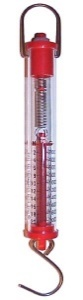
\includegraphics[scale=0.5,angle=90]{../figures/NewtonsLaws/scale}};
\draw[line width=1.5] (\hval,0) --+(\L,0);
\draw[line width=1.5] (-\hval,0) --+(-\L,0);
\fill (0,\R) circle(3pt);

\fill[black!50] (-\L-\hval,-\R) circle(\R);
\fill (-\L-\hval,-\R) circle(3pt);
\draw[line width=1.5] (-\hval-\L-\R,-\R) --+(0,-\L);
\fill[black!50] (-\hval-\L-1.5*\R,-\R-\L) rectangle (-\hval-\L-0.5*\R,-2*\R-\L);
\node at  (-\hval-\L-\R,-1.5*\R-\L) {$m$};
\fill (-\hval-\L-2.5*\R,-1.5*\R-\L) circle(3pt);

\fill[black!50] (\L+\hval,-\R) circle(\R);
\fill (+\L+\hval,-\R) circle(3pt);
\draw[line width=1.5] (\hval+\L+\R,-\R) --+(0,-\L);
\fill[black!50] (\hval+\L+1.5*\R,-\R-\L) rectangle (\hval+\L+0.5*\R,-2*\R-\L);
\node at  (\hval+\L+\R,-1.5*\R-\L) {$m$};
\fill (\hval+\L+2.5*\R,-1.5*\R-\L) circle(3pt);

}
\end{tikzpicture}
\captionof*{figure}{\textit{Two masses, two pulleys and a spring scale.}}
\end{center}
}



%%%%%%%%%%%%%%%%%%%%%%%%%%%%%%%%
%%%%%%%%%%%%%%%%%%%%%%%%%%%%%%%%
\twocolframe{Group exercise: Draw the FBDs for masses and scale}
{
\begin{itemize}
\item All forces have the same magnitude, but the pulleys change the direction of tension forces in the ropes.
\item The forces exerted on the scale are the same as in the previous problem, so it reads the same!
\item The Earth exerts the two forces of gravity (in red).
\end{itemize}
}
{

\begin{center}
\begin{tikzpicture}[scale=1]
\tikzmath{
\L=1.5;
\R=0.5;
\f=0.75;
}
\pgfmathsetmacro{\hval}{0.85}
\scalebox{1.0}{
\node at (0,0) {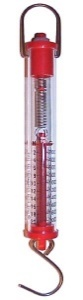
\includegraphics[scale=0.5,angle=90]{../figures/NewtonsLaws/scale}};
\draw[line width=1.5] (\hval,0) --+(\L,0);
\draw[line width=1.5] (-\hval,0) --+(-\L,0);
\fill (0,\R) circle(3pt) node[above]{\scriptsize Forces exerted by ropes on scale};
\draw [-latex,line width=1.5] (0,\R)  -- +(\f,0) ; 
\draw [-latex,line width=1.5] (0,\R)  -- +(-\f,0); 

\fill[black!50] (-\L-\hval,-\R) circle(\R);
\fill (-\L-\hval,-\R) circle(3pt);
\draw[line width=1.5] (-\hval-\L-\R,-\R) --+(0,-\L);
\fill[black!50] (-\hval-\L-1.5*\R,-\R-\L) rectangle (-\hval-\L-0.5*\R,-2*\R-\L);
\node at  (-\hval-\L-\R,-1.5*\R-\L) {$m$};
\fill (-\hval-\L-2.5*\R,-1.5*\R-\L) circle(3pt);
\draw [-latex,line width=1.5] (-\hval-\L-2.5*\R,-1.5*\R-\L)   -- +(0,\f) ; 
\draw [-latex,line width=1.5,color=myred] (-\hval-\L-2.5*\R,-1.5*\R-\L)   -- +(0,-\f); 


\fill[black!50] (\L+\hval,-\R) circle(\R);
\fill (+\L+\hval,-\R) circle(3pt);
\draw[line width=1.5] (\hval+\L+\R,-\R) --+(0,-\L);
\fill[black!50] (\hval+\L+1.5*\R,-\R-\L) rectangle (\hval+\L+0.5*\R,-2*\R-\L);
\node at  (\hval+\L+\R,-1.5*\R-\L) {$m$};
\fill (\hval+\L+2.5*\R,-1.5*\R-\L) circle(3pt);
\draw [-latex,line width=1.5] (\hval+\L+2.5*\R,-1.5*\R-\L)   -- +(0,\f); 
\draw [-latex,line width=1.5,color=myred] (\hval+\L+2.5*\R,-1.5*\R-\L)   -- +(0,-\f); 

}
\end{tikzpicture}
\captionof*{figure}{\textit{Two masses, two pulleys and a spring scale}}
\end{center}
}



%%%%%%%%%%%%%%%%%%%%%%%%%%%%%%%%



%%%%%%%%%%%%%%%%%%%%%%%%%%%%%%%%
\subsection{Newton's first law}
\label{subsec:newtonsfirstlaw}
\begin{frame}{Newton's first law}
\textbf{An object will remain in its state of motion, be it at rest or moving with constant velocity, unless a net external force is exerted on the object.}\\
\vfill
If the above is true, then you're observing the object from an inertial frame of reference. Think of this as the way to define an inertial frame of reference.
\end{frame}


%%%%%%%%%%%%%%%%%%%%%%%%%%%%%%%%
\subsection{Newton's second law}
\label{subsec:newtonssecondlaw}
\begin{frame}{Newton's Second Law}
\begin{align*}
\sum \vec F = m\vec a
\end{align*}
\begin{itemize}
\item This statement is a quantitative framework that describes almost all of the world around us. It leads to the concepts of conservation of energy, momentum, angular momentum, etc. It is an amazing equation!
\item It connects dynamics (forces) to kinematics (acceleration).
\item It is a vector equation $\rightarrow$ To be ``useful'' we need to write it out in components. 
\end{itemize}
\end{frame}

%%%%%%%%%%%%%%%%%%%%%%%%%%%%%%%%
\subsection{Newton's third law}
\label{subsec:newtonsthirdlaw}
\begin{frame}{Newton's third law}
\textbf{If one object exerts a force on another object, the second object
exerts a force on the first object that is equal in magnitude and
opposite in direction.}\\
\vfill
This is not about intuition!!! \textcolor{myred}{This is a rule to be followed!} (science)\\
\vfill
If you include a force on object A that is exerted by object B, then you need to include an equal and opposite force exerted on object B from object A (if you care about modeling the motion of object B).
\end{frame}


%%%%%%%%%%%%%%%%%%%%%%%%%%%%%%%%



%%%%%%%%%%%%%%%%%%%%%%%%%%%%%%%%



%%%%%%%%%%%%%%%%%%%%%%%%%%%%%%%%



%%%%%%%%%%%%%%%%%%%%%%%%%%%%%%%%



%%%%%%%%%%%%%%%%%%%%%%%%%%%%%%%%



%%%%%%%%%%%%%%%%%%%%%%%%%%%%%%%%



%%%%%%%%%%%%%%%%%%%%%%%%%%%%%%%%



%%%%%%%%%%%%%%%%%%%%%%%%%%%%%%%%



%%%%%%%%%%%%%%%%%%%%%%%%%%%%%%%%



%%%%%%%%%%%%%%%%%%%%%%%%%%%%%%%%



%%%%%%%%%%%%%%%%%%%%%%%%%%%%%%%%



%%%%%%%%%%%%%%%%%%%%%%%%%%%%%%%%

\end{document}